\documentclass{beamer}


\usetheme{Boadilla}
\usecolortheme{default}

\setbeamerfont{title}{series=\bfseries,parent=structure}
\setbeamerfont{frametitle}{series=\bfseries,parent=structure}

\usepackage{tikz}

\setbeamertemplate{background}{\tikz{
    \foreach \x in {-5,...,5} \draw (\x ,-5) -- (\x ,5) node[anchor=north] {$\x$};
    \foreach \y in {-5,...,5} \draw (-5,\y) -- (5,\y) node[anchor=east] {$\y$};}}
\begin{document}

\begin{frame}
  \frametitle{Titre de la frame}
  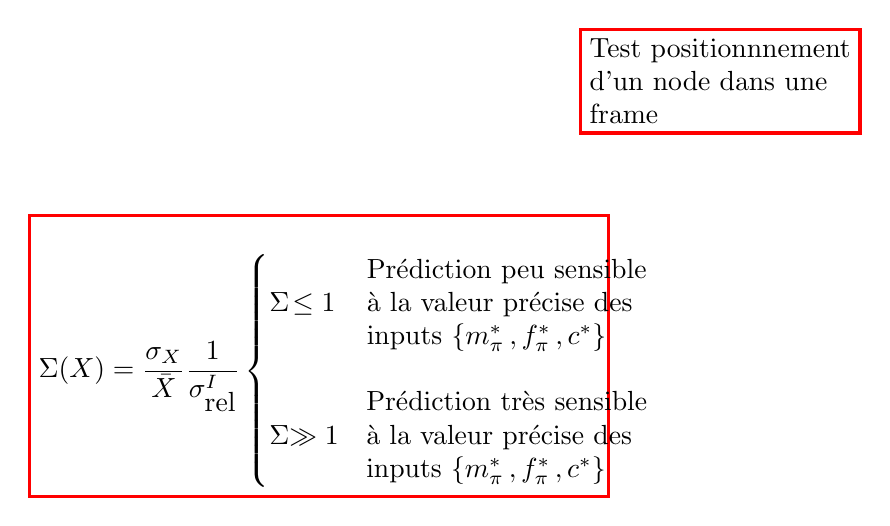
\begin{tikzpicture}
  %\draw (current page.south west) to[grid with coordinates] (current page.north east);
\node[rectangle,very thick,anchor=south west,align=left,draw=red] 
  at (2,2) {Test positionnnement \\ d'un node dans une \\ frame} ;
\node[rectangle,very thick,anchor=north west,align=left,draw=red] 
  at (-5,1) 
  {
    \begin{minipage}{7cm}
      \[
      \Sigma(X) =
    \frac{\sigma_X}{\bar{X}}\frac{1}{\sigma_{\textrm{rel}}^I}
    \left\{
      \begin{array}{@{}c@{}cc@{}}
        \Sigma & \le 1 & 
        \begin{array}{@{}l@{}}
          \textrm{Prédiction peu sensible}\\
          \textrm{à la valeur précise des} \\ 
          \textrm{inputs }\{m_\pi^*\,,f_\pi^*\,,c^*\}
        \end{array} \\ 
        && \\
        \Sigma & \gg 1 & 
        \begin{array}{@{}l@{}}
          \textrm{Prédiction très sensible}\\
          \textrm{à la valeur précise des }\\ 
          \textrm{inputs } \{m_\pi^*\,,f_\pi^*\,,c^*\}
        \end{array}\\ 
      \end{array}
    \right.
      \]
    \end{minipage}
  };
\end{tikzpicture}

\end{frame}

\end{document}